% questions.tex —— 1998 年·全国卷·文科 · 题目内容片段（无答案）
% 由 tools/generate_projects.py 依来源总账自 1998/1998_数学真题_全国文_试题.md 生成，勿手改（改源 MD 后重跑）


\gkpart{文科数学}

\begin{gktip}
\textbf{来源说明}：本题面依据固定源 PDF《1998 普通高等学校招生考试（全国卷文）》逐题转录。固定源为 1 页 A3 横向题面，原卷印刷页码 57；PDF 不含答案或解析页，下列答案和解析由本库独立推导，不声称代表官方发布版本。

\textbf{图形说明}：第 2、11、22、23、24 题的原卷图形关系重绘为 TikZ/PGFPlots 矢量图。图形标记所指的 PNG 不随仓库保存。
\end{gktip}

\begin{question}
\gkti{1}$\sin600^\circ$ 的值是\mbox{（　　）}

（A）$\dfrac12$　　（B）$-\dfrac12$　　（C）$\dfrac{\sqrt3}2$　　（D）$-\dfrac{\sqrt3}2$

\Needspace{0.4\textheight}
\end{question}
\begin{question}
\gkti{2}函数 $y=a^{|x|}\ (a>1)$ 的图象是\mbox{（　　）}
\nopagebreak[4]
\begin{center}\begin{tikzpicture}[x=1cm,y=1cm,line cap=round,line join=round]
\newcommand{\axes}{\draw[->] (-1.05,0)--(1.05,0) node[right] {$x$};\draw[->] (0,-0.12)--(0,1.18) node[above] {$y$};}
\begin{scope}
  \axes
  \draw[thick] plot[smooth] coordinates {(-0.75,1.02) (-0.48,0.42) (-0.2,0.10) (0,0) (0.2,0.10) (0.48,0.42) (0.75,1.02)};
  \node at (0,-0.38) {(A)};
\end{scope}
\begin{scope}[xshift=2.8cm]
  \axes
  \draw[densely dotted] (-0.08,0.36)--(0.08,0.36) node[right] {$1$};
  \draw[thick] plot[smooth] coordinates {(-0.78,1.02) (-0.48,0.55) (-0.2,0.39) (0,0.36) (0.2,0.39) (0.48,0.55) (0.78,1.02)};
  \node at (0,-0.38) {(B)};
\end{scope}
\begin{scope}[yshift=-2.1cm]
  \axes
  \draw[densely dotted] (-0.08,0.72)--(0.08,0.72) node[right] {$1$};
  \draw[thick] (-0.78,0.15) .. controls (-0.4,0.54) and (-0.16,0.72) .. (0,0.72)
    .. controls (0.16,0.72) and (0.4,0.54) .. (0.78,0.15);
  \node at (0,-0.38) {(C)};
\end{scope}
\begin{scope}[xshift=2.8cm,yshift=-2.1cm]
  \axes
  \draw[densely dotted] (-0.08,0.36)--(0.08,0.36) node[right] {$1$};
  \draw[thick] (-0.78,1.02) .. controls (-0.45,0.68) and (-0.18,0.40) .. (0,0.36)
    .. controls (0.18,0.40) and (0.45,0.68) .. (0.78,1.02);
  \node at (0,-0.38) {(D)};
\end{scope}
\end{tikzpicture}
\end{center}
\nopagebreak[4]
\end{question}
\begin{question}
\gkti{3}已知直线 $x=a\ (a>0)$ 和圆 $(x-1)^2+y^2=4$ 相切，那么 $a$ 的值是\mbox{（　　）}

（A）5　　（B）4　　（C）3　　（D）2

\end{question}
\begin{question}
\gkti{4}两条直线 $A_1x+B_1y+C_1=0$，$A_2x+B_2y+C_2=0$ 垂直的充要条件是\mbox{（　　）}

（A）$A_1A_2+B_1B_2=0$　　（B）$A_1A_2-B_1B_2=0$

（C）$\dfrac{A_1A_2}{B_1B_2}=-1$　　（D）$\dfrac{B_1B_2}{A_1A_2}=1$

\end{question}
\begin{question}
\gkti{5}函数 $f(x)=\dfrac1x\ (x\ne0)$ 的反函数 $f^{-1}(x)=$\mbox{（　　）}

（A）$x\ (x\ne0)$　　（B）$\dfrac1x\ (x\ne0)$

（C）$-x\ (x\ne0)$　　（D）$-\dfrac1x\ (x\ne0)$

\end{question}
\begin{question}
\gkti{6}已知点 $P(\sin\alpha-\cos\alpha,\tan\alpha)$ 在第一象限，则在 $[0,2\pi]$ 内 $\alpha$ 的取值范围是\mbox{（　　）}

（A）$\left(\dfrac\pi2,\dfrac{3\pi}4\right)\cup\left(\pi,\dfrac{5\pi}4\right)$

（B）$\left(\dfrac\pi4,\dfrac\pi2\right)\cup\left(\pi,\dfrac{5\pi}4\right)$

（C）$\left(\dfrac\pi2,\dfrac{3\pi}4\right)\cup\left(\dfrac{5\pi}4,\dfrac{3\pi}2\right)$

（D）$\left(\dfrac\pi4,\dfrac\pi2\right)\cup\left(\dfrac{3\pi}4,\pi\right)$

\end{question}
\begin{question}
\gkti{7}已知圆锥的全面积是底面积的 3 倍，那么该圆锥的侧面展开图扇形的圆心角为\mbox{（　　）}

（A）$120^\circ$　　（B）$150^\circ$　　（C）$180^\circ$　　（D）$240^\circ$

\end{question}
\begin{question}
\gkti{8}复数 $-\mathrm{i}$ 的一个立方根是 $\mathrm{i}$，它的另外两个立方根是\mbox{（　　）}

（A）$\dfrac{\sqrt3}2\pm\dfrac12\mathrm{i}$　　（B）$-\dfrac{\sqrt3}2\pm\dfrac12\mathrm{i}$

（C）$\pm\dfrac{\sqrt3}2+\dfrac12\mathrm{i}$　　（D）$\pm\dfrac{\sqrt3}2-\dfrac12\mathrm{i}$

\end{question}
\begin{question}
\gkti{9}如果棱台的两底面积分别是 $S,S'$，中截面的面积是 $S_0$，那么\mbox{（　　）}

（A）$2\sqrt{S_0}=\sqrt{S}+\sqrt{S'}$　　（B）$S_0=\sqrt{SS'}$

（C）$2S_0=S+S'$　　（D）$S_0^2=2SS'$

\end{question}
\begin{question}
\gkti{10}2 名医生和 4 名护士被分配到 2 所学校为学生体检，每校分配 1 名医生和 2 名护士，不同的分配方法共有\mbox{（　　）}

（A）6 种　　（B）12 种　　（C）18 种　　（D）24 种

\Needspace{0.4\textheight}
\end{question}
\begin{question}
\gkti{11}向高为 $H$ 的水瓶中注水，注满为止，如果注水量 $V$ 与水深 $h$ 的函数关系的图象如下图所示，那么水瓶的形状是\mbox{（　　）}
\nopagebreak[4]
\begin{center}\begin{tikzpicture}[x=1cm,y=1cm,line cap=round,line join=round]
% V(h) increases with decreasing slope; the dashed line marks h=H.
\draw[->] (0,0)--(2.1,0) node[right] {$h$};
\draw[->] (0,0)--(0,1.65) node[above] {$V$};
\draw[dashed] (1.55,0)--(1.55,1.35);
\draw[thick] (0,0) .. controls (0.20,0.9) and (0.55,1.2) .. (1.55,1.35);
\node[below left] at (0,0) {$O$};
\node[below] at (1.55,0) {$H$};

% Four schematic vessel profiles, with dashed rear halves of the rims/bases.
\newcommand{\bottle}[4]{%
  \begin{scope}[shift={(#1,0)}]
    \draw[thick] (#2,0.25)--(#3,1.45);
    \draw[thick] (-#2,0.25)--(-#3,1.45);
    \draw[thick] (0,1.45) ellipse [x radius=#3,y radius=0.12];
    \draw[thick] (-#2,0.25) arc[start angle=180,end angle=360,x radius=#2,y radius=0.09];
    \draw[dashed] (#2,0.25) arc[start angle=0,end angle=180,x radius=#2,y radius=0.09];
    \node[below] at (0,-0.05) {#4};
  \end{scope}}
\bottle{3.0}{0.28}{0.47}{(A)}
\bottle{4.25}{0.47}{0.28}{(B)}
\begin{scope}[shift={(5.5,0)}]
  \draw[thick] (-0.47,1.45) .. controls (-0.35,1.0) and (-0.2,0.82) .. (-0.28,0.25);
  \draw[thick] (0.47,1.45) .. controls (0.35,1.0) and (0.2,0.82) .. (0.28,0.25);
  \draw[thick] (0,1.45) ellipse [x radius=0.47,y radius=0.12];
  \draw[thick] (-0.28,0.25) arc[start angle=180,end angle=360,x radius=0.28,y radius=0.09];
  \draw[dashed] (0.28,0.25) arc[start angle=0,end angle=180,x radius=0.28,y radius=0.09];
  \node[below] at (0,-0.05) {(C)};
\end{scope}
\begin{scope}[shift={(6.8,0)}]
  \draw[thick] (-0.36,0.25)--(-0.36,1.45);
  \draw[thick] (0.36,0.25)--(0.36,1.45);
  \draw[thick] (0,1.45) ellipse [x radius=0.36,y radius=0.12];
  \draw[thick] (-0.36,0.25) arc[start angle=180,end angle=360,x radius=0.36,y radius=0.09];
  \draw[dashed] (0.36,0.25) arc[start angle=0,end angle=180,x radius=0.36,y radius=0.09];
  \node[below] at (0,-0.05) {(D)};
\end{scope}
\end{tikzpicture}
\end{center}
\nopagebreak[4]
\end{question}
\begin{question}
\gkti{12}椭圆

\nopagebreak[4]
\[
\frac{x^2}{12}+\frac{y^2}{3}=1
\]

的焦点为 $F_1$ 和 $F_2$，点 $P$ 在椭圆上，如果线段 $PF_1$ 的中点 $M$ 在 $y$ 轴上，那么点 $M$ 的纵坐标是\mbox{（　　）}

（A）7 倍　　（B）5 倍　　（C）4 倍　　（D）3 倍

\end{question}
\begin{question}
\gkti{13}球面上有 3 个点，其中任意两点的球面距离都等于大圆周长的 $\dfrac16$，经过这 3 个点的小圆的周长为 $4\pi$，那么这个球的半径为\mbox{（　　）}

（A）$\pm\dfrac{\sqrt3}4$　　（B）$\pm\dfrac{\sqrt2}2$　　（C）$\pm\dfrac{\sqrt3}2$　　（D）$\pm\dfrac34$

\end{question}
\begin{question}
\gkti{14}一个直角三角形三内角的正弦值成等比数列，其最小内角的正弦值为\mbox{（　　）}

（A）$\dfrac{1-\sqrt5}2$　　（B）$\dfrac{\sqrt5-1}2$　　（C）$\dfrac{\sqrt{2\sqrt5-2}}2$　　（D）$\dfrac{\sqrt{2\sqrt5+2}}2$

\end{question}
\begin{question}
\gkti{15}等比数列 $\{a_n\}$ 的公比为 $-\dfrac12$，前 $n$ 项和为 $S_n$，满足 $\lim\limits_{n\to\infty} S_n = \dfrac{1}{a_1}$，那么 $a_1$ 的值为\mbox{（　　）}

（A）$\pm\sqrt3$　　（B）$\pm\dfrac32$　　（C）$\pm\sqrt2$　　（D）$\pm\dfrac{\sqrt6}2$

\end{question}
\begin{question}
\gkti{16}设圆过双曲线

\nopagebreak[4]
\[
\frac{x^2}{9}-\frac{y^2}{16}=1
\]

的一个顶点和一个焦点，圆心在此双曲线上，则圆心到双曲线中心的距离是\gkblank{}。

\end{question}
\begin{question}
\gkti{17}$(x+2)^{10}(x^2-1)$ 的展开式中 $x$ 的系数为\gkblank{}。（用数字作答）

\end{question}
\begin{question}
\gkti{18}在直四棱柱 $A_1B_1C_1D_1-ABCD$ 中，当底面四边形 $ABCD$ 满足条件\gkblank{}时，有 $A_1C\perp B_1D_1$。（注：填上你认为正确的一种条件即可，不必考虑所有可能的情形）

\end{question}
\begin{question}
\gkti{19}关于函数

\nopagebreak[4]
\[
f(x)=4\sin\left(2x+\frac\pi3\right)\quad (x\in\mathbf{R}),
\]

有下列命题：

① 由 $f(x_1)=f(x_2)=0$ 可得 $x_1-x_2$ 必是 $\pi$ 的整数倍；

② $y=f(x)$ 的表达式可改写为 $y=4\cos\left(2x-\dfrac\pi6\right)$；

③ $y=f(x)$ 的图象关于点 $\left(-\dfrac\pi6,0\right)$ 对称；

④ $y=f(x)$ 的图象关于直线 $x=-\dfrac\pi6$ 对称。

其中正确的命题的序号是\gkblank{}。（注：把你认为正确的命题的序号都填上）

\end{question}
\begin{question}
\gkti{20}设 $a\ne b$，解关于 $x$ 的不等式：

\nopagebreak[4]
\[
a^2x+b^2(1-x)\ge [ax+b(1-x)]^2.
\]

\end{question}
\begin{question}
\gkti{21}在 $\triangle ABC$ 中，$a,b,c$ 分别是角 $A,B,C$ 的对边，设 $a+c=2b$，$A-C=\dfrac\pi3$，求 $\sin B$ 的值。

\Needspace{0.4\textheight}
\end{question}
\begin{question}
\gkti{22}如图，直线 $l_1$ 和 $l_2$ 相交于点 $M$，$l_1\perp l_2$，点 $N\in l_1$。以 $A,B$ 为端点的曲线段 $C$ 上的任一点到 $l_2$ 的距离与到点 $N$ 的距离相等。若 $\triangle AMN$ 为锐角三角形，$|AM|=\sqrt{17}$，$|AN|=3$，且 $|BN|=6$。建立适当的坐标系，求曲线段 $C$ 的方程。
\nopagebreak[4]
\begin{center}\begin{tikzpicture}[scale=0.48,line cap=round,line join=round]
\draw[->] (-0.6,0)--(7.0,0) node[right] {$l_1$};
\draw[->] (0,-0.25)--(0,6.45) node[above] {$l_2$};
\draw[thick,domain=3:6,samples=60,variable=\x] plot (\x,{sqrt(8*\x-16)});
\fill (0,0) circle (2pt) node[below left] {$M$};
\fill (4,0) circle (2pt) node[below] {$N$};
\fill (3,{sqrt(8)}) circle (2pt) node[left] {$A$};
\fill (6,{sqrt(32)}) circle (2pt) node[above right] {$B$};
\end{tikzpicture}
\end{center}
\nopagebreak[4]
\Needspace{0.4\textheight}
\end{question}
\begin{question}
\gkti{23}已知斜三棱柱 $ABC-A_1B_1C_1$ 的侧面 $A_1ACC_1$ 与底面 $ABC$ 垂直，$\angle ABC=90^\circ$，$BC=2$，$AC=2\sqrt3$，且 $AA_1\perp A_1C$，$AA_1=A_1C$。

（1） 求侧棱 $A_1A$ 与底面 $ABC$ 所成角的大小；

（2） 求侧面 $A_1ABB_1$ 与底面 $ABC$ 所成二面角的大小；

（3） 求侧棱 $B_1B$ 和侧面 $A_1ACC_1$ 的距离。
\nopagebreak[4]
\begin{center}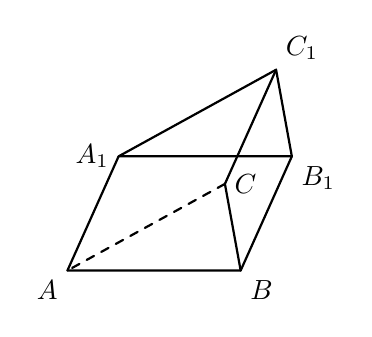
\begin{tikzpicture}[x=1cm,y=1cm,line cap=round,line join=round]
\coordinate (A) at (0,0);
\coordinate (B) at (2.2,0);
\coordinate (C) at (2.0,1.1);
\coordinate (Aone) at (0.65,1.45);
\coordinate (Bone) at (2.85,1.45);
\coordinate (Cone) at (2.65,2.55);
\draw[thick] (A)--(B)--(C);
\draw[thick,dashed] (C)--(A);
\draw[thick] (Aone)--(Bone)--(Cone)--cycle;
\draw[thick] (A)--(Aone) (B)--(Bone) (C)--(Cone);
\node[below left] at (A) {$A$};
\node[below right] at (B) {$B$};
\node[right] at (C) {$C$};
\node[left] at (Aone) {$A_1$};
\node[below right] at (Bone) {$B_1$};
\node[above right] at (Cone) {$C_1$};
\end{tikzpicture}
\end{center}
\nopagebreak[4]
\Needspace{0.4\textheight}
\end{question}
\begin{question}
\gkti{24}如图，为处理含有某种杂质的污水，要制造一底宽为 2 米的无盖长方体沉淀箱，污水从 $A$ 孔流入，经沉淀后从 $B$ 孔流出。设箱体的长度为 $a$ 米，高度为 $b$ 米。已知流出的水中该杂质的质量分数与 $a,b$ 的乘积 $ab$ 成反比。现有制箱材料 60 平方米。问当 $a,b$ 各为多少米时，经沉淀后流出的水中该杂质的质量分数最小。（$A$、$B$ 孔的面积忽略不计）
\nopagebreak[4]
\begin{center}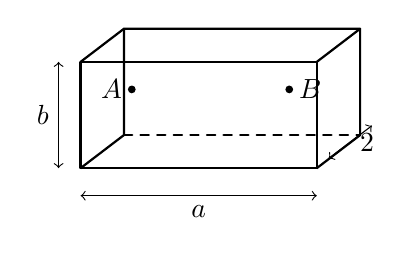
\begin{tikzpicture}[x=1cm,y=1cm,line cap=round,line join=round]
\coordinate (A) at (0,0);
\coordinate (B) at (3.0,0);
\coordinate (C) at (3.0,1.35);
\coordinate (D) at (0,1.35);
\coordinate (Aback) at (0.55,0.42);
\coordinate (Bback) at (3.55,0.42);
\coordinate (Cback) at (3.55,1.77);
\coordinate (Dback) at (0.55,1.77);
\draw[thick] (A)--(B)--(C)--(D)--cycle;
\draw[thick] (D)--(Dback)--(Cback)--(C);
\draw[thick] (A)--(Aback)--(Dback);
\draw[thick] (B)--(Bback)--(Cback);
\draw[thick,dashed] (Aback)--(Bback);
\fill (0.65,1.0) circle (1.4pt) node[left] {$A$};
\fill (2.65,1.0) circle (1.4pt) node[right] {$B$};
\draw[<->] (0,-0.35)--(3,-0.35) node[midway,below] {$a$};
\draw[<->] (-0.28,0)--(-0.28,1.35) node[midway,left] {$b$};
\draw[<->] (3.15,0.12)--(3.7,0.54) node[midway,right] {$2$};
\end{tikzpicture}
\end{center}
\nopagebreak[4]
\end{question}
\begin{question}
\gkti{25}已知数列 $\{b_n\}$ 是等差数列，$b_1=1$，$b_1+b_2+\cdots+b_{10}=145$。

（1） 求数列 $\{b_n\}$ 的通项 $b_n$；

（2） 设数列 $\{a_n\}$ 的通项 $a_n=\lg\left(1+\dfrac{1}{b_n}\right)$（其中 $a>0$，且 $a\ne 1$），记 $S_n$ 是数列 $\{a_n\}$ 的前 $n$ 项和。试比较 $S_n$ 与 $\dfrac12\lg b_n + 1$ 的大小，并证明你的结论。

\end{question}